\section{Background and Preliminary}
\label{sec:background}
UPPRESSO is compatible with OIDC and provides privacy protection based on the discrete logarithm problem. Here, we provide a brief introduction about OIDC and the discrete logarithm problem.

\subsection{OpenID Connect (OIDC)}
\label{subsec:OIDC}
As an extension of OAuth 2.0 to support user authentication, OIDC~\cite{OpenIDConnect} is one of the most prominent SSO authentication protocols. Same as other SSO protocols~\cite{SAMLIdentifier}, OIDC involves three entities, i.e., {\em users}, {\em identity provider (IdP)}, and {\em relying parties (RPs)}.
Both users and RPs have to register at the IdP with identifiers such as $ID_U$ and $ID_{RP}$ (or $PID_{RP}$ in some schemes) and the corresponding account information such as credential, RP's endpoint (e.g., URLs), etc.
% below can be removed
IdP is assumed to maintain these attributes securely. In an OIDC authentication session, a user is responsible for initiating a login request at an RP, redirecting the SSO messages between the RP and IdP, and checking the scope of the user attributes in the identify proof generated by the IdP for the RP. Usually, the redirection and checking actions are handled by a user-controlled software, known as {\em user agent} (e.g., browser). Once receiving a user login request, the RP constructs an identity proof request with its identifier and the requested scope of  user's attributes, sends an identity proof request to the IdP through the user, and parses the received identity proof to authenticate and authorize the user. The IdP authenticates the user based on her $ID_U$ and credential, sets the $PPID$ (i.e., a privacy-preserving pseudo-identifier) for the user-RP pair (denoted by $ID_U$ and $ID_{RP}$), generates an identity proof containing $PPID$, $ID_{RP}$ and the user attributes, and returns the identity proof to the endpoint registered by the RP.

\vspace{1mm}\noindent\textbf{OIDC implicit flow.} OIDC supports three different SSO authentication processes (called flows), which are the {\em implicit flow}, {\em authorization code flow} and {\em hybrid flow} (i.e., a mix-up of the previous two). In the implicit flow, an {\em id token} is generated as the identity proof, which contains user identifier (i.e., $PPID$), RP identifier (i.e., $ID_{RP}$), the issuer (i.e., IdP), issuing time, the validity period, and other requested attributes. The IdP signs the id token using its private key to ensure integrity, and sends it to RP through the user. In the authorization code flow, the IdP binds an authorization code with the RP, and sends it to the RP through the user; then, the RP establishes an HTTPS connection to the IdP %to ensure the integrity and confidentiality of the identity proof,
and uses the authorization code with the RP's credential to obtain user's PPID and other attributes.
UPPRESSO is compatible with all three flows. For brevity, we will present our design and implementation of UPPRESSO on top of the implicit flow of OIDC in details, and discuss the extension to support the authorization code flow in Section~\ref{sec:discussion}.

The protocol flow of the original OIDC implicit flow is shown in Figure~\ref{fig:OpenID}, consisting of 7 steps: when a user attempts to log in to an RP (Step 1), the RP constructs an identity proof request and returns it to the user, which gets redirected to the IdP (Step 2). The request contains $ID_{RP}$, RP's endpoint and a set of requested user attributes. If the user has not yet been authenticated, the IdP initiates an authentication process (Step 3) to authenticate the user. For a successfully authenticated user, the IdP generates an id token (Step 4) and returns it to the registered endpoint of the RP (Step 5). If no registered endpoint is found for that RP, the IdP will generate a warning to notify the user about potential identity proof leakage. Once the RP receives the id token, it verifies its signature (Step 6) and makes the authentication decision (Step 7).
%extracts user's identifier and returns the authentication result to the user (Step 7).

\vspace{1mm}\noindent\textbf{RP dynamic registration.} OIDC has a dynamic registration mechanism~\cite{DynamicRegistration} that allows an RP to update its information at the IdP dynamically. When an RP first registers at the IdP, it obtains a registration token, with which the RP can invoke a dynamic registration process to update its information (e.g., the endpoint). After a successful dynamic registration, the RP obtains a new and unique $ID_{RP}$ from the IdP. UPPRESSO leverages this function and slightly modify the dynamic registration process to enable {\em RP identifier refreshing}, which allows each RP to generate different privacy-preserving identifiers ($PID_{RP}$s) and register them at the IdP.

\begin{figure}[t]
  \centering
  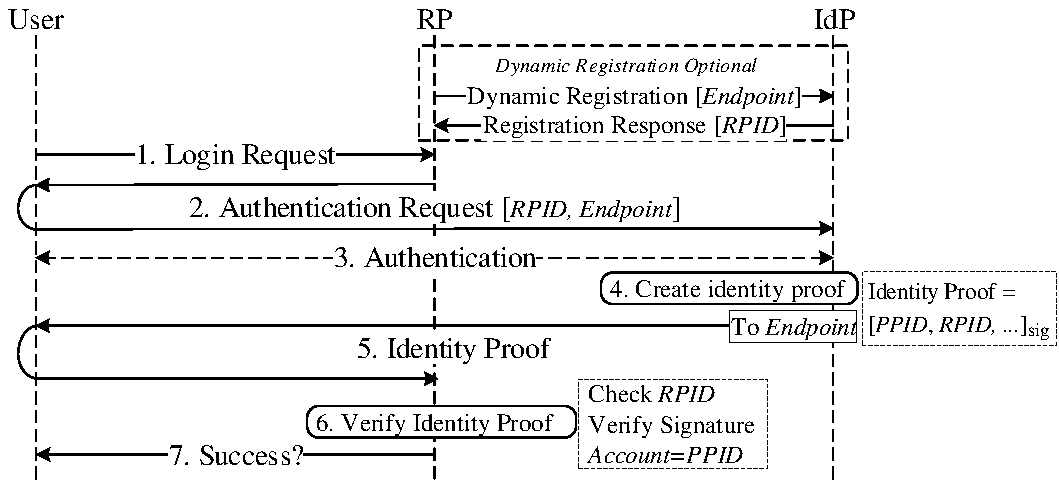
\includegraphics[width=\linewidth]{fig/OIDC1.pdf}
  \caption{The implicit flow of OIDC.}
  \label{fig:OpenID}
\end{figure}

\subsection{Discrete Logarithm Problem}
\label{sec:dlp}

Based on the discrete logarithm problem, UPPRESSO design the identifier-transformation functions $\mathcal{F}_{ID_{RP} \mapsto PID_{RP}}$ and $\mathcal{F}_{ID_{U} \mapsto PID_{U}}$ to generate privacy-preserving user identifier (e.g. $PID_U$) and RP identifier (e.g. $PID_{RP}$), respectively. Here, we briefly review the discrete logarithm problem.

%A number $g$ ($0<g<p$) is called a primitive root modular a prime $p$, if for ${\forall}y$ ($0<y<p$), there is a  number $x$ ($0\le x <p-1$) satisfying $y=g^x \pmod p$.
For $GF(p)$ where $p$ is a large prime, a number $g$ is called a generator of order $q$, if it can be used to construct a cyclic  group of $q$ elements by calculating $y=g^x \ mod\ p$.
And, $x$ is called the discrete logarithm of $y$ modulo $p$. Given a large prime $p$, a generator $g$ and a number $y$, it is computationally infeasible to derive the discrete logarithm (here $x$) of $y$ (detailed in~\cite{WXWM}), which is called the discrete logarithm problem. The hardness of solving discrete logarithm has been used to construct several security primitives, including Diffie-Hellman key exchange and Digital Signature Algorithm (DSA).

%In the process of $F_{PID_{RP}}$ and $F_{PID_U}$, we needs to calculate the primitive root for a  large prime $p$ as follows~\cite{Shoup,Wang}. First, we retrieve a primitive root $g_m$  modulo $p$ from all the integers by finding the first integer passing  the primitive root checking.  A lemma is propose to simply the checking, that if $p=2q+1$ ($q$ is a prime),  an integer $\mu \in (1, p-1)$ is a primitive root if and only if $\mu^2\neq 1 \ mod \ p$ and $\mu^q\neq 1 \ mod \ p$. Then, based on $g_m$, we can calculate a new primitive root $g = g_{m}^{t} mod \ p$, where $t$ is an integer coprime to $p-1$.
